\section{Značaj podataka u dubokom učenju}
Prvi i najdulji praktični korak treninga predstavlja priprema podataka. 
Sve ovisi o zadatku koji mreža mora riješiti, ali, generalno je pravilo da je više podataka bolje.
Konačna kvaliteta rješenja osim o arhitekturi mreže koju dizajniramo, ovisi o kvaliteti podataka kojom ju usmjeravamo.
Priprema podataka vrši se u 3 glavna koraka (\cite{generalDatasets}):
\begin{enumerate}
\item Prikupljanje
\item Klasifikacija
\item Označavanje
\end{enumerate} 
\subsubsection{Prikupljanje podataka}
Prikupljanje podataka mora biti sustavan i smislen proces jer može otežati i olakšati daljnje korake. 
Najpreporučeniji način za prikupljanje je dugoročno i postepeno spremanje podataka jer rezultira velikim brojem objektivnih i kvalitetih podataka.
Ja sam se ipak odlučio na metodu računalnog generiranja vlastitog seta podataka. 
Razlog tome je raznolikost elemenata koje mreža mora moći detektirati i fleksibilnost koju dobivam jednomo kada ustanovim sve potrebe.
\subsubsection{Klasifikacija i označavanje podataka}
Generirani podaci na određeni način moraju biti prikazani mreži. 
Iako u mrežu slika ulazi kao vektor dimenzija \texttt{(visina x širina x kanali)} mreži su potrebni i podaci za uspoređivanje rezultata i računanje uspješnosti.
U ovom radu koristio sa \texttt{.csv} datoteku za dohvaćanje i opisnik slika. 
Postupak automatskog generiranja slika uvelike je olakšao klasifikaciju i označavanje jer je cijeli postupak ostvaren kao "cjevovod".
Pri izlasku, slika bi bila prikazana kao na slici ~\ref{fig:pipelineExitExample}.
Datoteka bi upisano imala ime slike, simbol na slici, širinu, visinu i točan položaj elementa na slici. 
Prednost ovog pristupa je i u tom što slika nije zadana absolutnom putanjom, što znači, da sam slike mogao kreirati na vlastitom računalu, prenjeti ih na udaljeni server za treniranje i bez komplikacija koristiti iste. \\
Veličina opisnika je također bila zanemariva. 
Nakon raspodjele \texttt{80:20} za trening i validaciju na 15 000 slika, veličine su bile \texttt{440kB} i \texttt{110kB} dok je direktorij sa slikama bio veličine \texttt{6,7GB}.

\begin{figure}[h!]
	\centering
	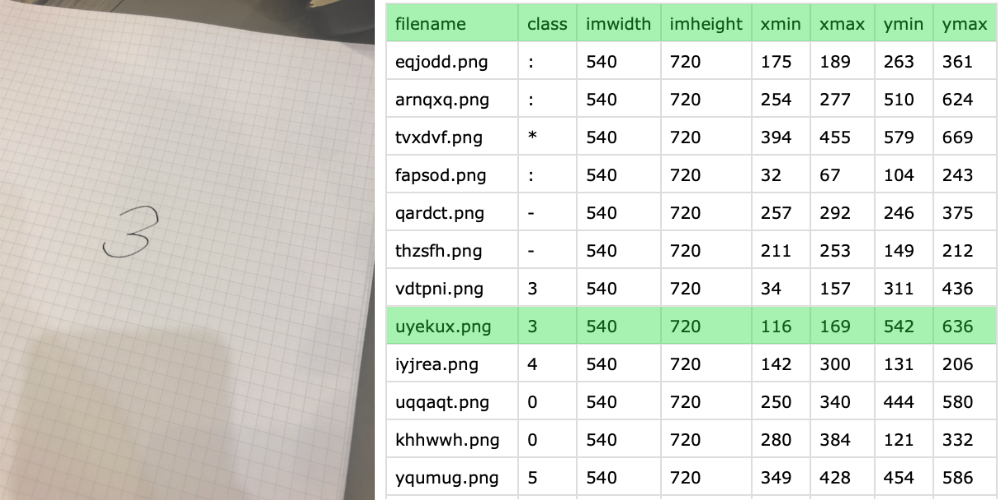
\includegraphics[width=1.0\linewidth]{image_csv}
	 \caption{Slika i pripadajuća referenca u .csv datoteci}
 	 \label{fig:pipelineExitExample}
\end{figure}

\section{Generiranje slika}
\subsection{Generalizacija postupka}
Za relativan uspjeh treniranja mreže za detekciju i klasifikaciju 14 tekstovnih elemenata (0-9, +, -, *, :) potrebno je minimalno 10 000 slika. Ne samo zbog broja elemenata već i zbog složenosti i raznolikosti između njih. 
Postupak koji sam razvio primjenjuje sve taktike (\cite{chollet2017deep}) potrebne za stvaranje raznovrsnog i kvalitetnog seta podataka.
Zbog transformacija, opisanih u daljnjim djelovima poglavlja, gotovo je nemoguće da iako se isti font stavlja na pozadinu, nastane isti oblik.
Na slici ~\ref{fig:imageGenerationPipeline} prikazana je topologija cjevovoda koja kreira slike.
Cijeli cjevovod, implementiran je unutar programskog paketa \emph{ImageGenerator}, kojeg sam napisao u svrhu apstraktiranja cijelog postupka.
\begin{figure}[h!]
	\centering
	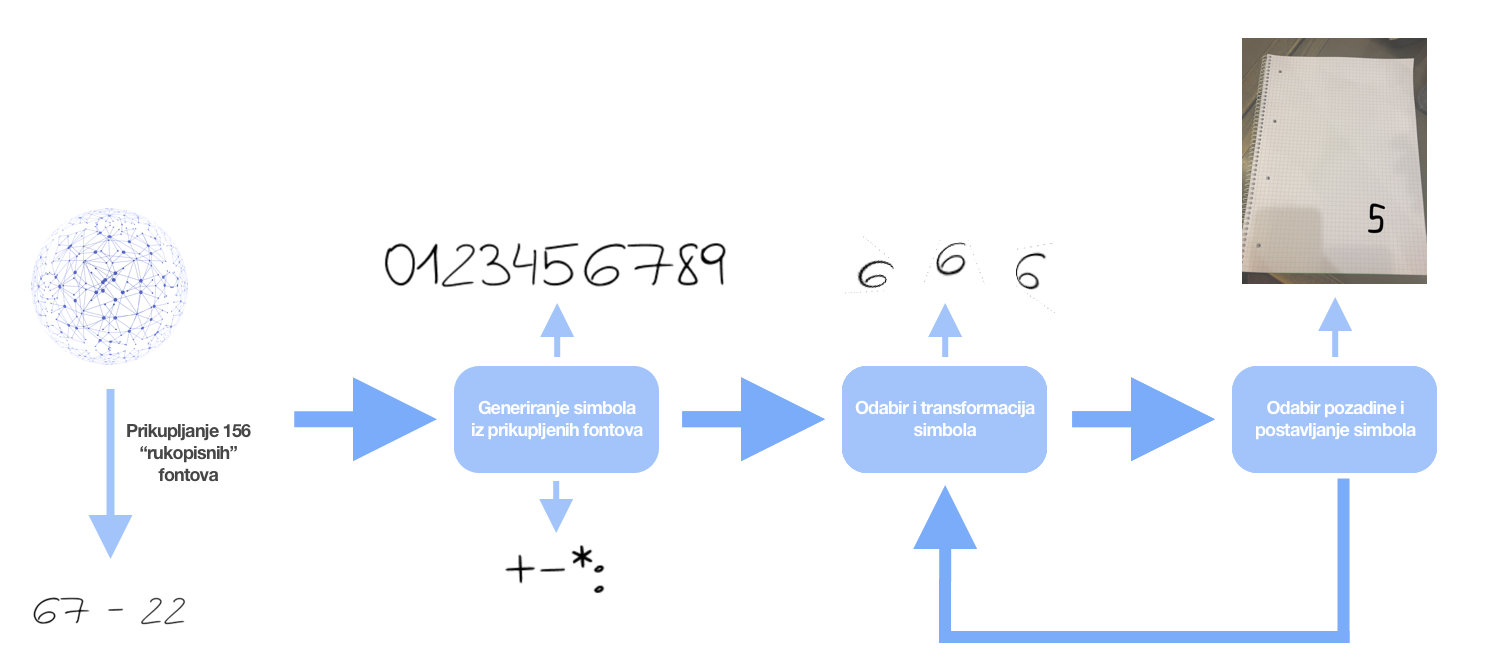
\includegraphics[width=1.0\linewidth]{image_generation_pipeline}
	 \caption{Prikaz visoke razine cjevovoda za generiranje slika}
 	 \label{fig:imageGenerationPipeline}
\end{figure}

\subsection{Prikupljanje fontova}
Ispisivanje velikog broja simbola sa razlikom između varijacija istog monoton je i neisplativ posao, posebice zbog dostupnosti svih potrebnih resursa na internetu.
U prilog je također išlo to što su dostupni fontovi, koji primjenjuju rukopisni stil, najčešće zbilja napisani rukom i vektorizirani, pa, generiranje i transformiranje neće negativno utjecati na kvalitetu.
Osim rukopisnih fontova, skinuo sam mali broj fontova koji su stilski između čistog rukopisnog i tipkanog.
Fontovi su bili prikupljeni sa sljedećih izvora, a na slici ~\ref{fig:fontDiffs} vidljivi su primjeri istih:
\begin{itemize}
\item \url{https://www.dafont.com}
\item \url{https://www.1001fonts.com}
\item \url{https://www.1001freefonts.com}
\end{itemize}
\begin{figure}[h!]
	\centering
	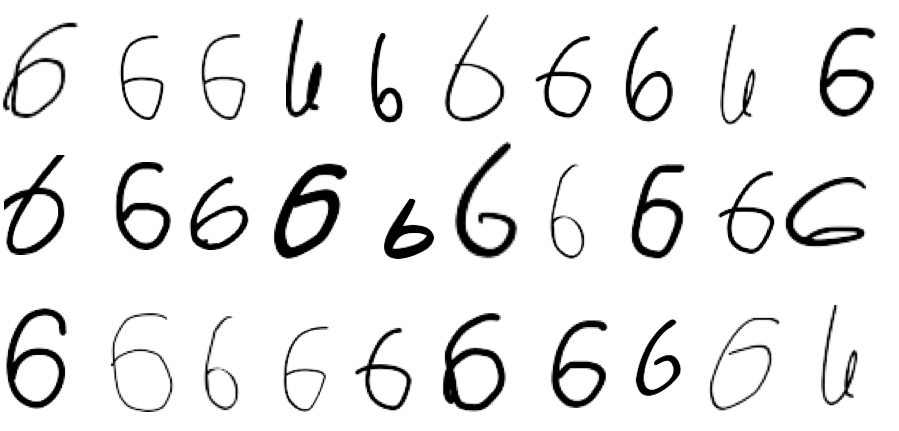
\includegraphics[width=0.85\linewidth]{font_diffs}
	 \caption{Varijacije unutar simbola uzrokovane fontovima}
 	 \label{fig:fontDiffs}
\end{figure}

\subsection{Generiranje simbola}
Nakon prikupljanja i sortiranja fontova, generiranje samih simbola bio je jednostavan posao.
Važno je bilo očuvati transparentnost pozadine iza simbola jer u trenutku kada se postavi na pozadinu po izboru, ona mora biti vidljiva.
\begin{algorithm}
\caption{Generiraj sve simbole}
\begin{algorithmic}[1]
	\Function{generirajTextSliku}{$font, simbol$}
		\State $velicina \gets font.velicina(simbol)$
		\State $slika \gets Image('RGBA', size, (255, 255, 255, 0))$
		\State $slika.text = simbol$
		
		\Return $slika$
	\EndFunction
	\Function{generirajSveSimbole}{\null}
		\For{\texttt{simbol in simboli}}
			\For{\texttt{i in [0, brojFontova>}}
				\State $direktorijSimbola \leftarrow spoji(putDoSimbola, simbol)$
				\If{$direktorijSimbola\ ne\ postoji$}
					\State \Call{kreirajDirektorij}{$direktorijSimbola$}
				\EndIf
				\State $font \leftarrow fontovi[i]$
				\State $generirana slika \gets$ \Call{generirajTextSliku}{$font, simbol$}
				\State \Call{spremiSliku}{$generiranaSlika$}
			\EndFor
		\EndFor
	\EndFunction
\end{algorithmic}
\end{algorithm}

\subsection{Transformacije}
\subsubsection{Skaliranje}
sdfadsf
\subsubsection{Rotacija}
fasdf
\subsubsection{Afine transfromacije}
asdfsadf
\subsection{Kreiranje cjelovitih slika}
afdfaf
